\documentclass[10pt]{article}
\usepackage[margin=1.5cm]{geometry}
\usepackage{graphicx,hyperref,booktabs,amsmath}
\hypersetup{colorlinks=true,urlcolor=blue}
\setlength{\parindent}{0pt}\setlength{\parskip}{6pt}
\begin{document}
\begin{center}
{\Large Full P-256 m2 ideal regularity: $198\to14$}\\[4pt]
17 November 2026 \quad Original depth 8 base \quad Unsigned local certificate
\end{center}
The fixed unplanted complete m2 system has ideal-module CM regularity 198
for GCB-dense and 14 for GCB-chain, under the same actual generator
homogenization. This is a full-system result, distinct from membership
regularity. Independent signed/Lean admission is pending. Claim
\texttt{PCC-20261117-644dc1}; standing \texttt{[pcc:unverified]}.

Curve:\\
\texttt{icv1-fp256-t89188191154553853111372247798585809583-f188c491}.\\
Factor base: \texttt{FB1h16882188194e},144 columns / 288 signed points. All
retained points and both signs preserved; original ICV1/FB1 wide codec.

\begin{center}
\begin{tabular}{lrr}\toprule
Fixed unplanted m2 & Dense & Chain\\\midrule
Affine variables & 4 & 18\\
Membership equations & 4 & 102\\
Group equations & 1 & 1\\
Input quotient regularity & 194 & 10\\
Full quotient regularity & 197 & 13\\
\textbf{Full ideal regularity D} & \textbf{198} & \textbf{14}\\
Full Artinian length & 331776 & 331776\\\bottomrule
\end{tabular}
\end{center}
Each has one common homogenizing variable. Same degree 4 complete group
circuit, same preselected target line, no affine-linear preprocessing and
no free slope/inverse/group witnesses. Added chain coordinates are unique.

\textbf{Exact proof.} Dense input is the retained strict CI(3,96) per point.
Chain input is an exact retained point ideal with 51 generators in 9 coordinates,
Hilbert numerator $[1,9,37,89,106,46]$ and quotient regularity 5. H-free
terminating border division, complete footprint and independent rank prove
the homogeneous point ideal, including over the algebraic closure.
No unexecuted S-pair loop is reported as passing.

Every $288^2=82944$ ordered m2 tuple is checked against GMP, RCB and
OpenSSL, for both frozen targets. Planted has exactly two ordered tuples
$(193,262),(262,193)$; unplanted has none. Zero false positives/negatives
on complete instances; both relations replayed, no independent-rank claim.

Therefore the common unplanted degree 4 polynomial is a nonzerodivisor on
both reduced dimension 1 CM input algebras. The regular-element sequence
gives the exact Artinian Hilbert polynomial
\[\operatorname{Hilb}(A/(f),t)=h_A(t)(1+t+t^2+t^3).\]
Its last degree is quotient regularity. Dense CI(3,96,3,96,4) Koszul shifts
agree with 197. Chain's last coefficient 2116 is in degree 13. Add 1 for ideal
regularity. The proof needs no general Gorenstein lower-bound lemma and
does not replace generator homogenization by saturation.

Both affine unplanted ideals are inconsistent. These regularities describe
their preregistered unsaturated homogenized generators; no affine F4 or
runtime gain is inferred. Native primary/fresh replay match byte-for-byte,
two corrupt controls rejected. The certificate remains unsigned.

\newpage
\begin{center}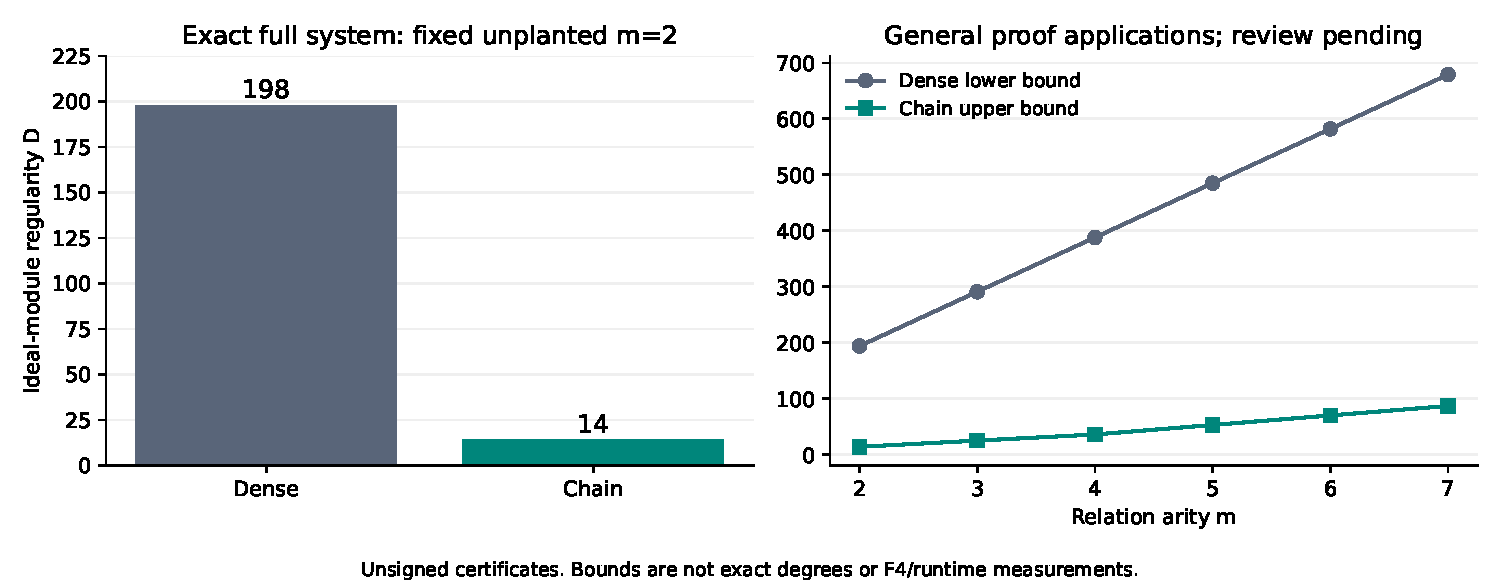
\includegraphics[width=\linewidth]{complete-comparison.pdf}\end{center}
\textbf{Preserved m2--7 scope.} Twelve paired planted/unplanted inputs,
six planted GMP/OpenSSL target replays and 2,862 membership equation checks.
Every reported relation is replayed. 129 complete-law controls cover identity,
doubling, inverses and nonunit projective scales; cubic gcd 1 excludes
rational 2-torsion. Twelve target-line nonsquare certificates are recorded.
Claim \texttt{PCC-20261117-08e7b0}; standing unsigned.

\texttt{FULL\_BOUND\_PROOF.md} supplies producer-derived general upper/lower
bounds, with the concrete chain quotient regularity 5:
\begin{center}\begin{tabular}{rrrr}\toprule
$m$ & Dense D lower & Chain D upper & Added affine variables\\\midrule
2&194&14&14\\3&291&25&21\\4&388&36&28\\5&485&53&35\\
6&582&70&42\\7&679&87&49\\\bottomrule
\end{tabular}\end{center}
Higher-m entries are bounds under the general proof, not measured exact
degrees. 1,024 finite-grid subset/degree controls test the duality shift,
not a universal theorem. Higher-m unplanted solving and independent proof
review remain open. Exact unplanted m2 above avoids that general lemma.

\textbf{Accounting and limits.} Seven added coordinates per point.
BM construction/check: 25,915,095 / 16,331,773 GMP modular-reduction API calls;
assembly/reference: 7,152,413 calls. These are setup/replay counts, not
field-equivalent solve operations. Circuits are not extra ring variables;
high-m coefficient expansion, solve time, RAM/disk traffic and EKS performance
remain unmeasured. No natural-yield, affine F4 or novelty claim.

New graph lift timed out at 30s with no result. Four older CoCoA cells remain
censored at 45s; exhausted public allowance was not reopened. Separate new
native correctness phases passed and replayed. No paid/performance run.

\textbf{Reproduce.} Run \texttt{bash run\_complete\_replay.sh FRESH\_DIR}.
This rebuilds the new package and compares its JSONs, excluding old failed
cells. Read \texttt{COMPLETE\_REPORT.md} and the four preregistered protocols.
The 2x numeric target is met locally; goal stays active for independent
admission and remaining full-scope obligations. No Rust/Lean executables
were available; their suites were not run.

\textbf{Sources.} RCB Algorithm1:
\url{https://joostrenes.nl/publications/complete.pdf}.
BM/filtered duality sources are linked in the Markdown report and native
protocols. Classical methods reused; no novelty claim. KB unavailable
(wrapper127), fallback literature review recorded. Standing unsigned.
\end{document}
